\newpage

\section{Anexos}

\FloatBarrier
\begin{figure}[H] 
				
			\centering
			
				\begin{subfigure}{.5\textwidth}
				  \centering
				  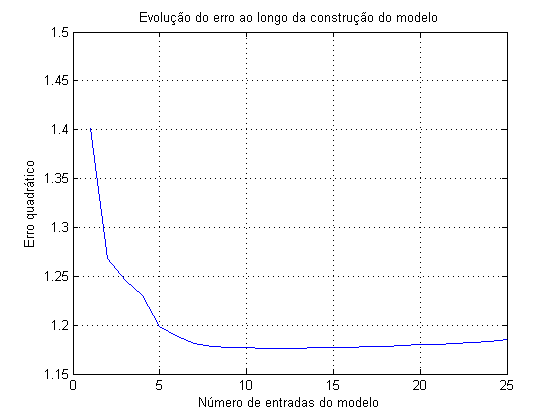
\includegraphics[width=1\linewidth]{image/forward1}
				  \caption{Resultado da execução 1.}
				  \label{forward1}
				\end{subfigure}%
				\begin{subfigure}{.5\textwidth}
				  \centering
				  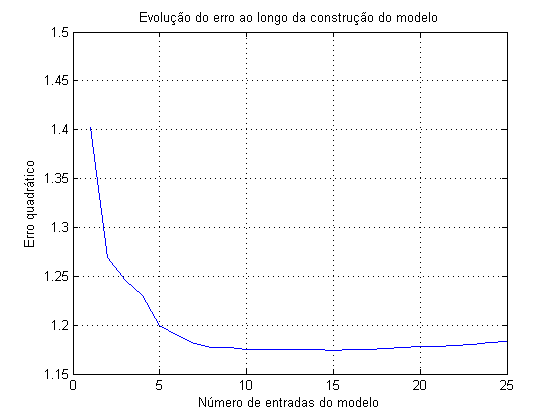
\includegraphics[width=1\linewidth]{image/forward2}
				  \caption{Resultado da execução 2.}
				  \label{forward2}
			\end{subfigure}
			
			\begin{subfigure}{.5\textwidth}
				  \centering
				  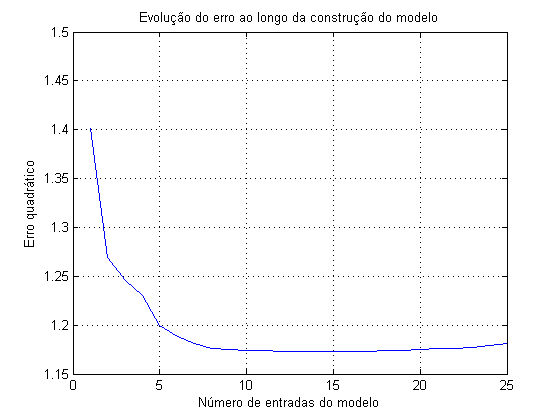
\includegraphics[width=1\linewidth]{image/forward3}
				  \caption{Resultado da execução 3.}
				  \label{forward3}
				\end{subfigure}%
				\begin{subfigure}{.5\textwidth}
				  \centering
				  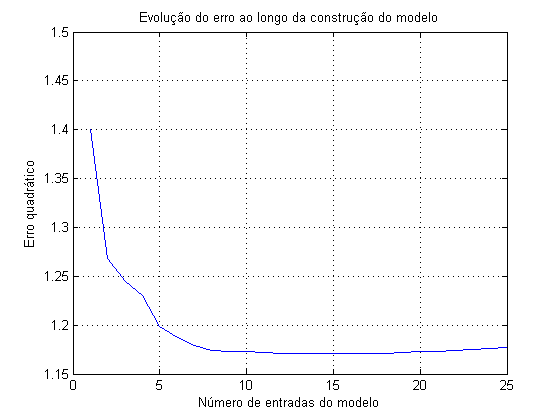
\includegraphics[width=1\linewidth]{image/forward4}
				  \caption{Resultado da execução 4.}
				  \label{forward4}
				\end{subfigure}			
			
			\begin{subfigure}{.5\textwidth}
				  \centering
				  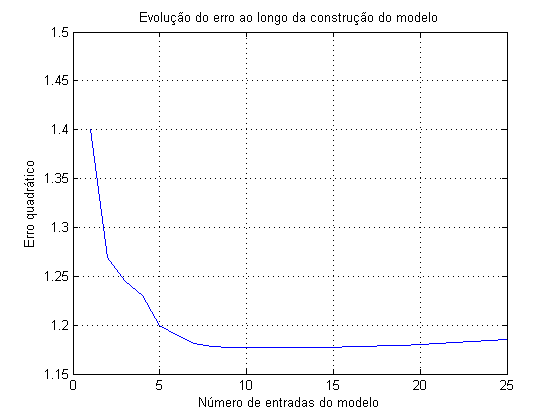
\includegraphics[width=1\linewidth]{image/forward5}
				  \caption{Resultado da execução 5.}
				  \label{forward5}
				\end{subfigure}	
			
			\caption{Resultados das execuções da \textit{forward selection} para os
			dados de \texttt{sunspot.mat}.}
			\label{fig:forw}
			\end{figure}
			
		\FloatBarrier
		
		\begin{figure}[H] 
				
			\centering
			
				\begin{subfigure}{.5\textwidth}
				  \centering
				  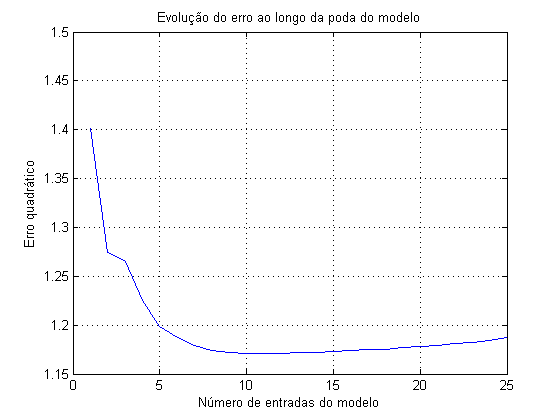
\includegraphics[width=1\linewidth]{image/backward1}
				  \caption{Resultado da execução 1.}
				  \label{backward1}
				\end{subfigure}%
				\begin{subfigure}{.5\textwidth}
				  \centering
				  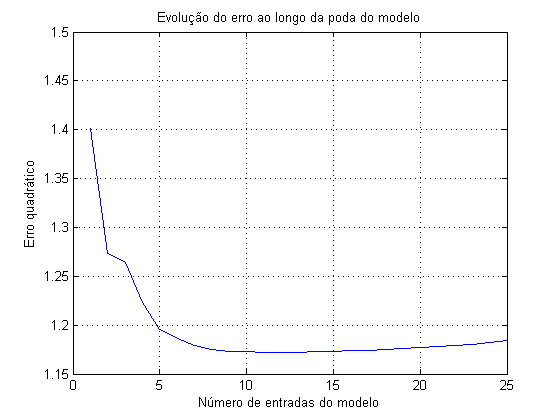
\includegraphics[width=1\linewidth]{image/backward2}
				  \caption{Resultado da execução 2.}
				  \label{backward2}
			\end{subfigure}
			
			\begin{subfigure}{.5\textwidth}
				  \centering
				  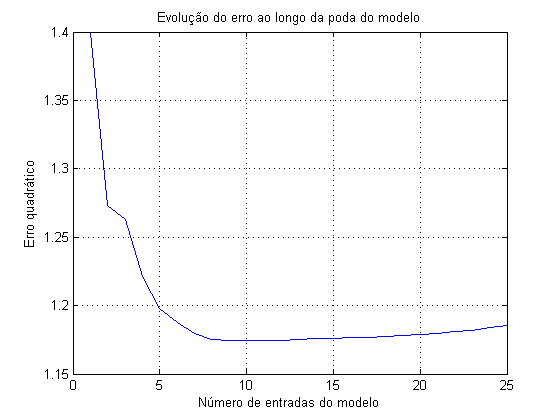
\includegraphics[width=1\linewidth]{image/backward3}
				  \caption{Resultado da execução 3.}
				  \label{backward3}
				\end{subfigure}%
				\begin{subfigure}{.5\textwidth}
				  \centering
				  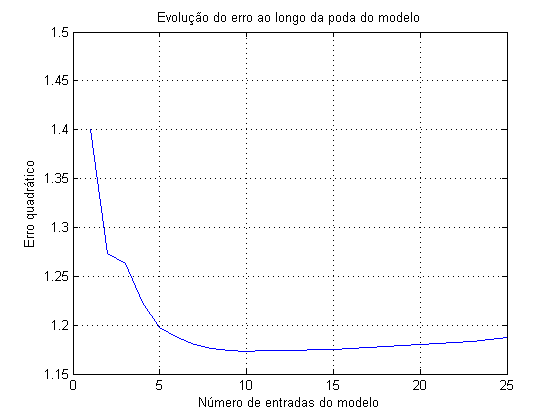
\includegraphics[width=1\linewidth]{image/backward4}
				  \caption{Resultado da execução 4.}
				  \label{backward4}
				\end{subfigure}			
			
			\begin{subfigure}{.5\textwidth}
				  \centering
				  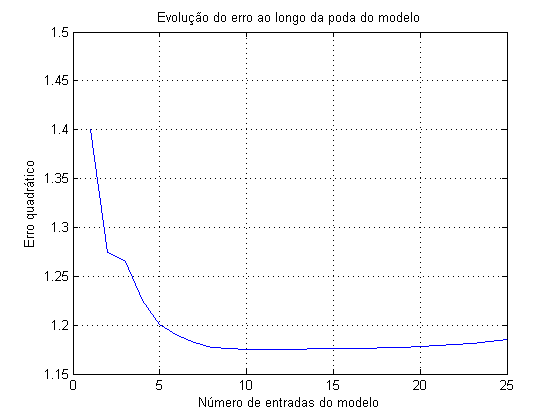
\includegraphics[width=1\linewidth]{image/backward5}
				  \caption{Resultado da execução 5.}
				  \label{backward5}
				\end{subfigure}	
			
			\caption{Resultados das execuções da \textit{backward elimination} para os
			dados de \texttt{sunspot.mat}.}
			\label{fig:back}
			\end{figure}


\FloatBarrier
\begin{figure}[H] 
				
			\centering
			
				\begin{subfigure}{.5\textwidth}
				  \centering
				  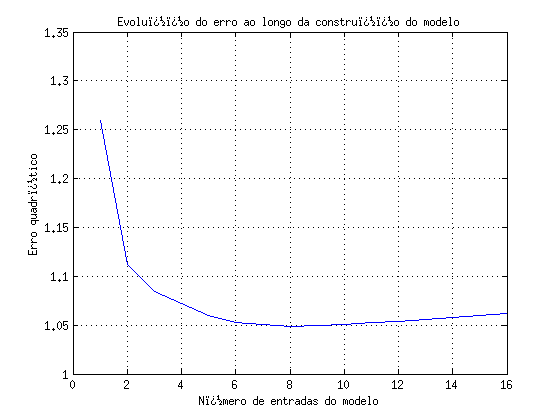
\includegraphics[width=1\linewidth]{image/forward1_2}
				  \caption{Resultado da execução 1.}
				  \label{forward1_2}
				\end{subfigure}%
				\begin{subfigure}{.5\textwidth}
				  \centering
				  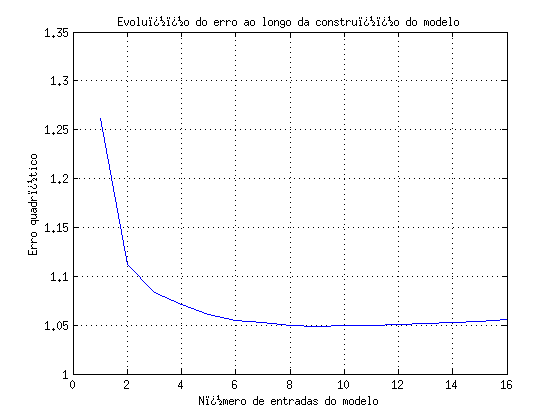
\includegraphics[width=1\linewidth]{image/forward2_2}
				  \caption{Resultado da execução 2.}
				  \label{forward2_2}
			\end{subfigure}
			
			\begin{subfigure}{.5\textwidth}
				  \centering
				  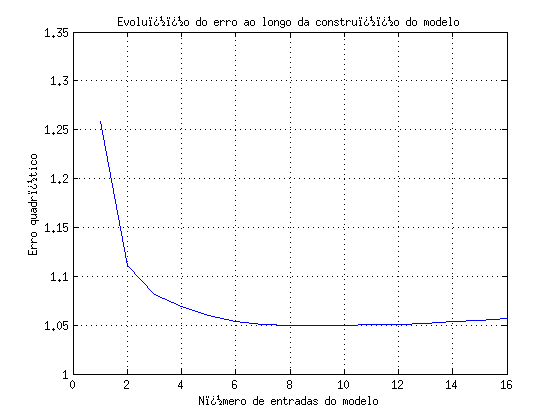
\includegraphics[width=1\linewidth]{image/forward3_2}
				  \caption{Resultado da execução 3.}
				  \label{forward3_2}
				\end{subfigure}%
				\begin{subfigure}{.5\textwidth}
				  \centering
				  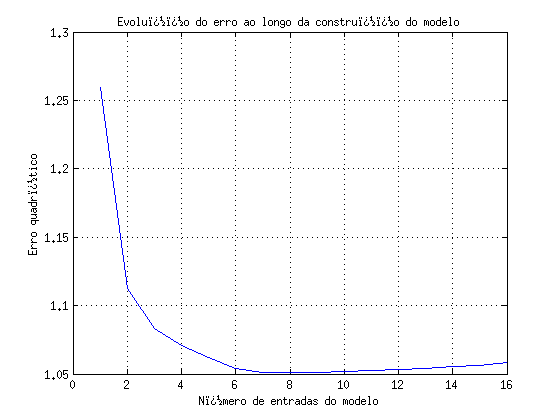
\includegraphics[width=1\linewidth]{image/forward4_2}
				  \caption{Resultado da execução 4.}
				  \label{forward4_2}
				\end{subfigure}			
			
			\begin{subfigure}{.5\textwidth}
				  \centering
				  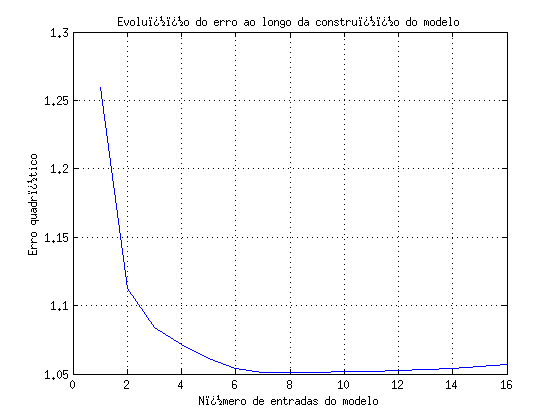
\includegraphics[width=1\linewidth]{image/forward5_2}
				  \caption{Resultado da execução 5.}
				  \label{forward5_2}
				\end{subfigure}	
			
			\caption{Resultados das execuções da \textit{forward selection} para os
			dados de \texttt{wineq.mat}.}
			\label{fig:forw2}
			\end{figure}
			
		\FloatBarrier
				
		\begin{figure}[H] 
				
			\centering
			
				\begin{subfigure}{.5\textwidth}
				  \centering
				  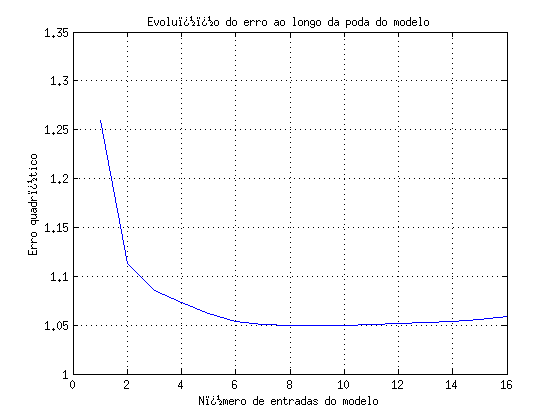
\includegraphics[width=1\linewidth]{image/backward1_2}
				  \caption{Resultado da execução 1.}
				  \label{backward1_2}
				\end{subfigure}%
				\begin{subfigure}{.5\textwidth}
				  \centering
				  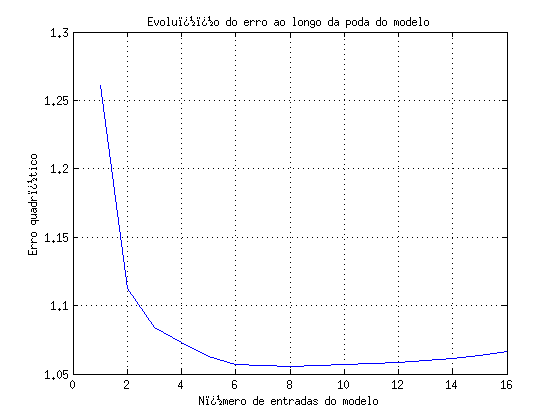
\includegraphics[width=1\linewidth]{image/backward2_2}
				  \caption{Resultado da execução 2.}
				  \label{backward2_2}
			\end{subfigure}
			
			\begin{subfigure}{.5\textwidth}
				  \centering
				  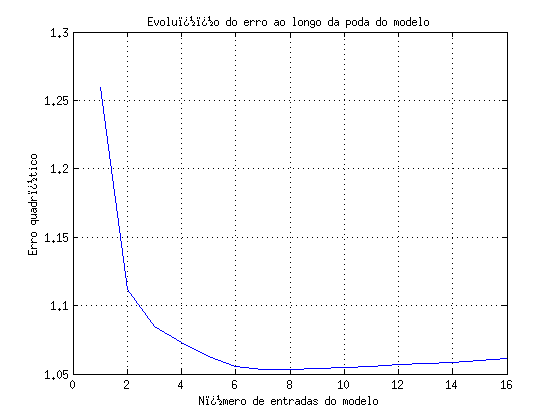
\includegraphics[width=1\linewidth]{image/backward3_2}
				  \caption{Resultado da execução 3.}
				  \label{backward3_2}
				\end{subfigure}%
				\begin{subfigure}{.5\textwidth}
				  \centering
				  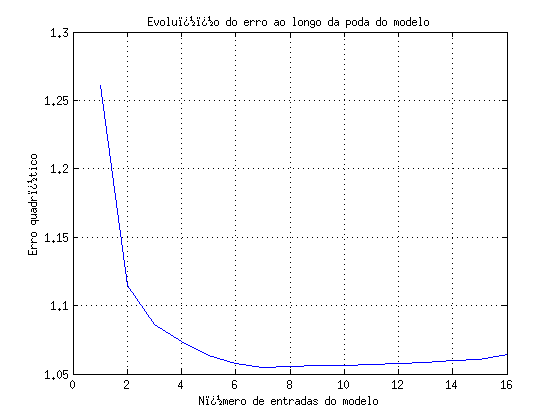
\includegraphics[width=1\linewidth]{image/backward4_2}
				  \caption{Resultado da execução 4.}
				  \label{backward4_2}
				\end{subfigure}			
			
			\begin{subfigure}{.5\textwidth}
				  \centering
				  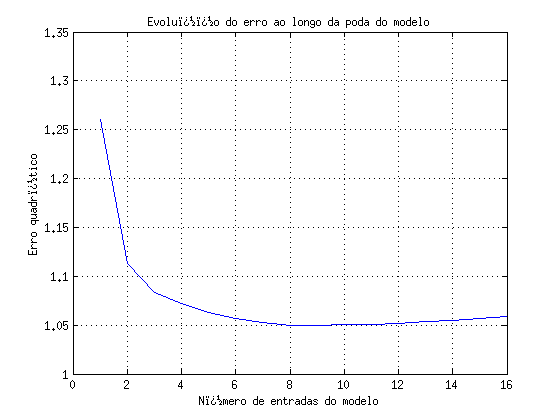
\includegraphics[width=1\linewidth]{image/backward5_2}
				  \caption{Resultado da execução 5.}
				  \label{backward5_2}
				\end{subfigure}	
			
			\caption{Resultados das execuções da \textit{backward elimination} para os
			dados de \texttt{wineq.mat}.}
			\label{fig:back2}
			\end{figure}
			
		\FloatBarrier
		
		\newpage
		
		\lstinputlisting [language=Matlab, caption={ \texttt{gera\_dados.m} - cria a
		sequência temporal.}, label={lst:geracao}] {predicao/gera_dados.m}
		
		\lstinputlisting [language=Matlab, caption={
		\texttt{resolve\_sistema\_k\_folds.m} - calcula preditores.},
		label={lst:preditor}] {predicao/resolve_sistema_k_folds.m}
		
		\lstinputlisting [language=Matlab, caption={ 
		\texttt{numberNeuronsMLP.m} - Automatiza treinamento e análise de redes MLP.},
		label={lst:mlp}] {predicao/numberNeuronsMLP.m}
		
		\FloatBarrier
		
		\begin{figure}[H] 
				
			\centering
			
				\begin{subfigure}{.33\textwidth}
				  \centering
				  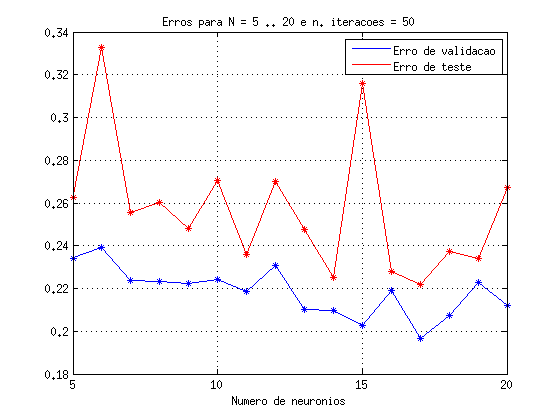
\includegraphics[width=1\linewidth]{image/mlp_50_iterations}
				  \caption{\(i=50\).}
				\end{subfigure}%
				\begin{subfigure}{.33\textwidth}
				  \centering
				  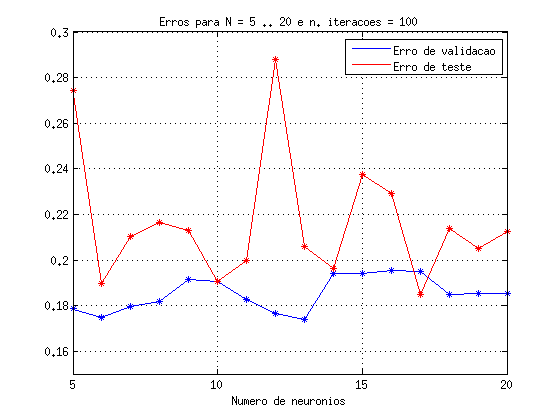
\includegraphics[width=1\linewidth]{image/mlp_100_iterations}
				  \caption{\(i=100\).}
			\end{subfigure}
			\begin{subfigure}{.33\textwidth}
				  \centering
				  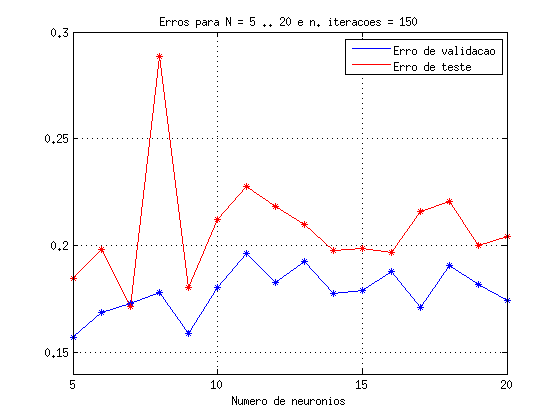
\includegraphics[width=1\linewidth]{image/mlp_150_iterations}
				  \caption{\(i=150\).}
				\end{subfigure}%
				
				\begin{subfigure}{.33\textwidth}
				  \centering
				  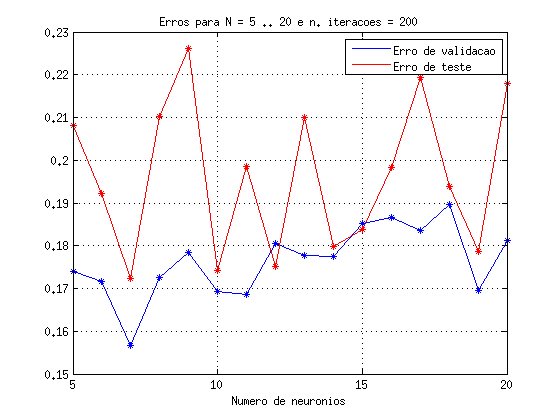
\includegraphics[width=1\linewidth]{image/mlp_200_iterations}
				  \caption{\(i=200\).}
				\end{subfigure}%
				\begin{subfigure}{.33\textwidth}
				  \centering
				  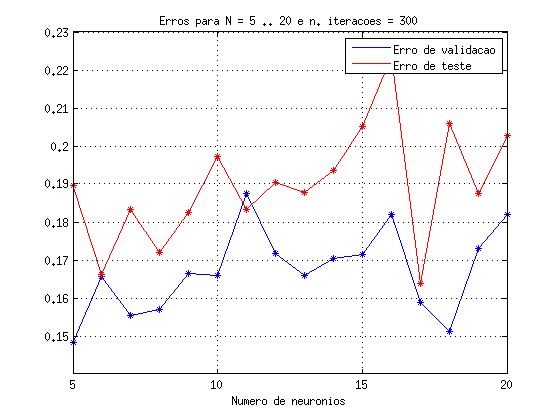
\includegraphics[width=1\linewidth]{image/mlp_300_iterations}
				  \caption{\(i=300\).}
			\end{subfigure}
			\begin{subfigure}{.33\textwidth}
				  \centering
				  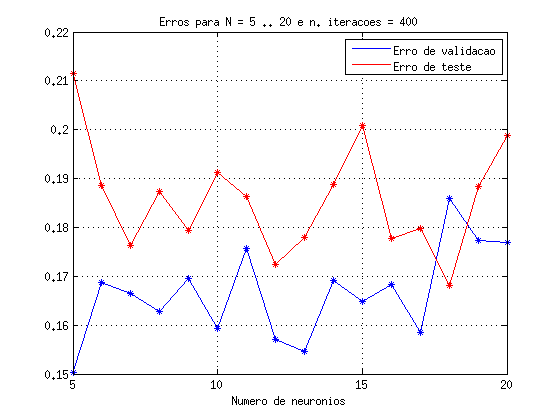
\includegraphics[width=1\linewidth]{image/mlp_400_iterations}
				  \caption{\(i=400\).}
				\end{subfigure}%	
				
			\begin{subfigure}{.33\textwidth}
				  \centering
				  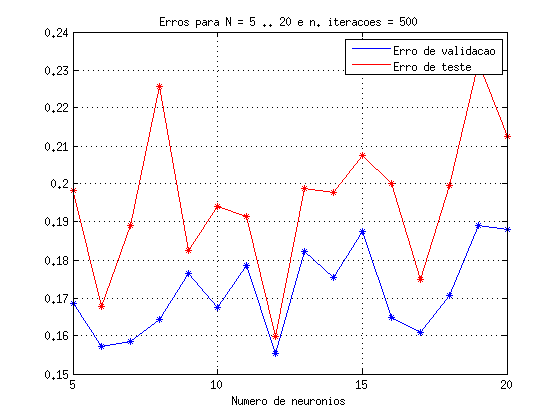
\includegraphics[width=1\linewidth]{image/mlp_500_iterations}
				  \caption{\(i=500\).}
				\end{subfigure}%
				\begin{subfigure}{.33\textwidth}
				  \centering
				  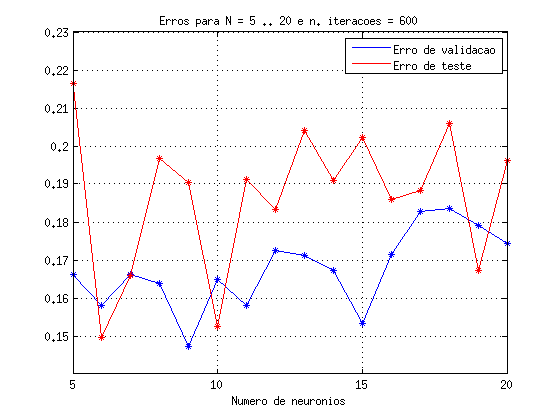
\includegraphics[width=1\linewidth]{image/mlp_600_iterations}
				  \caption{\(i=600\).}
			\end{subfigure}
			\begin{subfigure}{.33\textwidth}
				  \centering
				  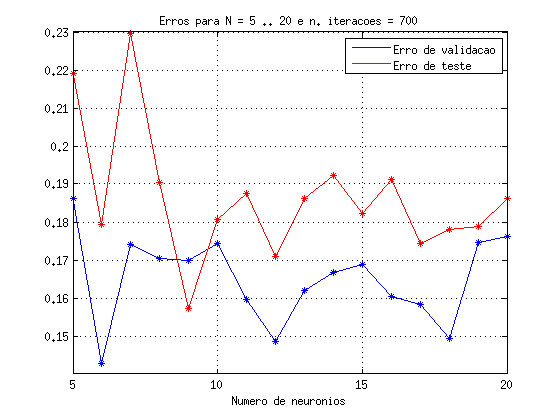
\includegraphics[width=1\linewidth]{image/mlp_700_iterations}
				  \caption{\(i=700\).}
				\end{subfigure}%
			
			\begin{subfigure}{.5\textwidth}
				  \centering
				  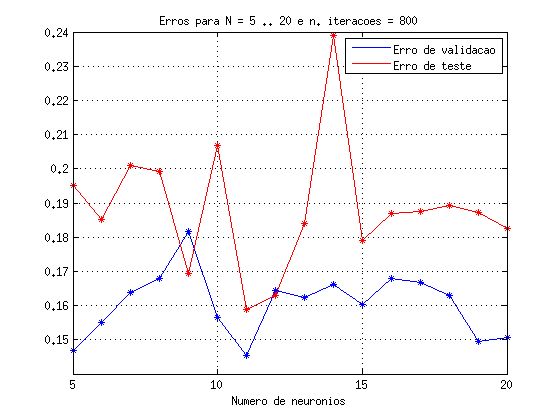
\includegraphics[width=1\linewidth]{image/mlp_800_iterations}
				  \caption{\(i=800\).}
				\end{subfigure}%
				\begin{subfigure}{.5\textwidth}
				  \centering
				  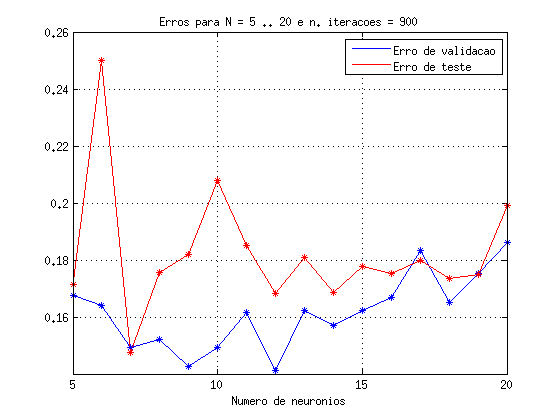
\includegraphics[width=1\linewidth]{image/mlp_900_iterations}
				  \caption{\(i=900\).}
			\end{subfigure}
			
			\caption{Médias dos erros de validação e de
			teste para vários valores possíveis \(i\) de iteração.}
			\end{figure}
			
		\FloatBarrier
		